\documentclass[12pt]{article}
\usepackage[hmargin=1in,vmargin=1in]{geometry}
\usepackage{amsmath,amssymb}
\usepackage{graphicx}
\usepackage{comment}
\usepackage{mathtools}
\usepackage{listings}
\usepackage{float}
\usepackage{fixltx2e}

\usepackage{subcaption}
\usepackage{epstopdf}


%opening
\title{EE239AS - Project 4}
\author{Yuxin Jin (104195828), Jamie Lee (604589757),\\ David Hong (204588953) and Nick Cirillo (103834979)}

\begin{document}

\maketitle


\section{Popularity Prediction on Twitter}

With the increase in popularity of social media and communication, Twitter has emerged as a major platform for online networking which allows users to post and read 140-character messages called tweets. Tweets are publicly viewable via the website and users can subscribe to other user's tweets in the form "following" another user. A word, phrase or topic that is mentioned at a greater rate than others is said to be a "trending topic" and can often be recognized in the form of hashtags ie. \#TrendingTopic. These topics  become popular usually either through a specific event or topic that prompts people to discuss it or by purely users creating these discussions. This information easily allows users to obtain broad perspectives and recent updates. In addition to users, these trending and bursting topics have sparked recent interest in the scientific community to analyze and predict these topics.

In this project we seek to analyze such data by utilizing current and previous tweet activity for given hashtags in order to predict future tweet activity and behavior. Specifically we analyze tweet data for the 2015 Super Bowl (Seattle Seahawks vs. New England Patriots) from a period of two weeks before the game to a week after the game. We will use from related hashtags to train a regression model and use the same model to make predictions for other hashtags.


\subsection{Part 1:}

The training data was downloaded and statistics were calculated for each of the hashtags (\#gohawks, \#gopatriots, \#nfl, \#patriots, \#sb49 and \#superbowl). We report data on each hashtag for the total number of tweets, average number of tweets per hour, average number of retweets and average number of followers per users. Statistics for each hashtag can be found in the tables below.

\begin{table}[h]
	\centering
	\begin{tabular}{| c | c | c | c |}
		\hline 
		Total \# of Tweets & 188135 \\\hline
		Avg. \# of Tweets per Hour & 276.669118 \\\hline
		Avg. \# of Retweets & 0.209164 \\\hline
		Avg \# of Followers of (77168) Users & 1720.634084 \\\hline
	\end{tabular} 
	\caption{\#gohawks statistics}
	\label{part1:tab1}
\end{table} 

\begin{table}[h]
	\centering
	\begin{tabular}{| c | c | c | c |}
		\hline 
		Total \# of Tweets & 26231 \\\hline
		Avg. \# of Tweets per Hour & 58.551339 \\\hline
		Avg. \# of Retweets & 0.026838 \\\hline
		Avg \# of Followers of (18005) Users & 1559.278200 \\\hline
	\end{tabular} 
	\caption{\#gopatriots statistics}
	\label{part1:tab1}
\end{table} 

\begin{table}[h]
	\centering
	\begin{tabular}{| c | c | c | c |}
		\hline 
		Total \# of Tweets & 259019 \\\hline
		Avg. \# of Tweets per Hour & 420.485390 \\\hline
		Avg. \# of Retweets & 0.050938 \\\hline
		Avg \# of Followers of (75167) Users & 4399.303205 \\\hline
	\end{tabular} 
	\caption{\#nfl statistics}
	\label{part1:tab1}
\end{table} 

\begin{table}[h]
	\centering
	\begin{tabular}{| c | c | c | c |}
		\hline 
		Total \# of Tweets & 489710 \\\hline
		Avg. \# of Tweets per Hour & 736.406015 \\\hline
		Avg. \# of Retweets & 0.091462 \\\hline
		Avg \# of Followers of (326173) Users & 1865.903974 \\\hline
	\end{tabular} 
	\caption{\#patriots statistics}
	\label{part1:tab1}
\end{table} 

\begin{table}[h]
	\centering
	\begin{tabular}{| c | c | c | c |}
		\hline 
		Total \# of Tweets & 826905 \\\hline
		Avg. \# of Tweets per Hour & 1531.305556 \\\hline
		Avg. \# of Retweets & 0.178023 \\\hline
		Avg \# of Followers of (590066) Users & 2247.285607 \\\hline
	\end{tabular} 
	\caption{\#sb49 statistics}
	\label{part1:tab1}
\end{table} 

\begin{table}[h]
	\centering
	\begin{tabular}{| c | c | c | c |}
		\hline 
		Total \# of Tweets & 1348766 \\\hline
		Avg. \# of Tweets per Hour & 2207.472995 \\\hline
		Avg. \# of Retweets & 0.136686 \\\hline
		Avg \# of Followers of (689690) Users & 4228.627878 \\\hline
	\end{tabular} 
	\caption{\#superbowl statistics}
	\label{part1:tab1}
\end{table} 


The total tweet count per hour both both the \#SuperBowl and the \#NFL hashtags are also shown below. Both hashtags noticeably show initial trending prior to the SuperBowl, show significant bursting during the SuperBowl event and both die relatively quickly after the SuperBowl (Feburary 1, 2015).

\begin{figure}
	\centering
	\begin{subfigure}{.45\textwidth}
		\centering
		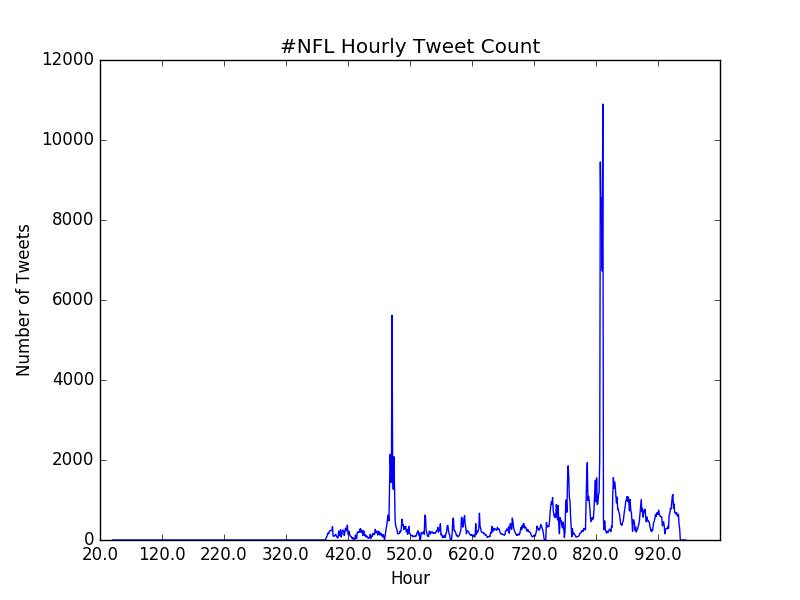
\includegraphics[width=\textwidth]{figures/1_NFL_histogram.jpeg}
		\centering
		\caption{\#NFL Hourly Tweet Count}
		\label{prob1:fig:1}
	\end{subfigure}%
	\hfill
	\begin{subfigure}{.45\textwidth}
		\centering
		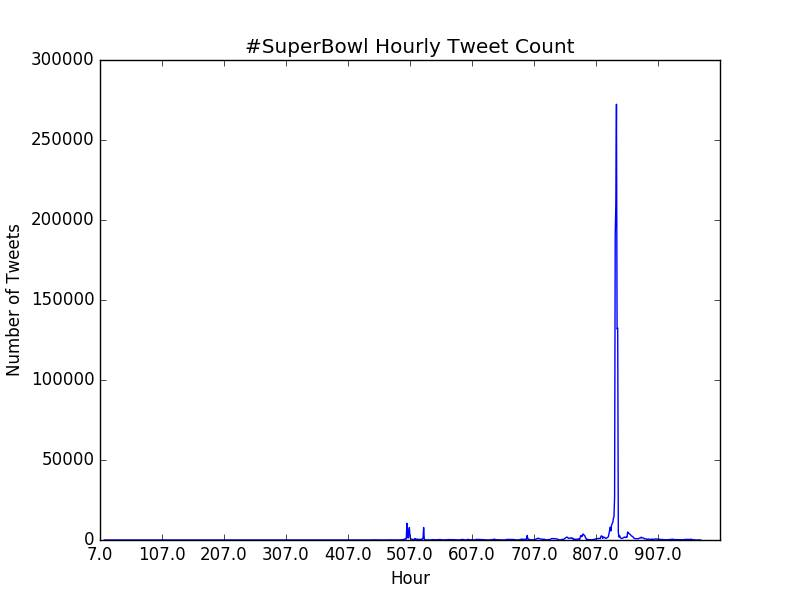
\includegraphics[width=\textwidth]{figures/1_SuperBowl_histogram.jpeg}
		\centering
		\caption{\#SuperBowl Hourly Tweet Count}
		\label{prob1:fig:2}
	\end{subfigure}
	\caption{Tweet counts per hour for tweet data obtained from 2 weeks prior to a week after the 2015 Superbowl}
\end{figure}

\subsection{Part 2:}



\end{document}